\documentclass[conference]{IEEEtran}

% -------------------------------------------------------
% Packages
% -------------------------------------------------------
\usepackage[utf8]{inputenc}
\usepackage{graphicx}
\graphicspath{{../figures/}}
\usepackage{amsmath}
\usepackage{amssymb}
\usepackage{booktabs}
\usepackage{float}
\usepackage{cite}
\usepackage{caption}
\usepackage{subcaption}
\usepackage{multirow}
\usepackage{url}
\usepackage{hyperref}

% -------------------------------------------------------
% Title, Authors, Affiliations
% -------------------------------------------------------
\title{Blood Pressure Analysis (USA): A Statistical and\\Machine Learning Approach}

\author{Ibrahim Ghauri \& Muhammad Mudassir\\
Department of Artificial Intelligence \& Data Science, School of Computing, FAST-NUCES\\
}

\begin{document}

\maketitle

% -------------------------------------------------------
% Abstract
% -------------------------------------------------------
\begin{abstract}
This study examines the predictive relationship between five cardiovascular risk factors---age, body mass index (BMI), cholesterol level, glucose level, and physical activity status---and systolic blood pressure (SBP) in a sample of 100 adults drawn from a publicly available cardiovascular health dataset. Two complementary modelling approaches are employed: Multiple Linear Regression (MLR), which provides interpretable coefficient estimates under linearity assumptions, and a Random Forest Regressor (RFR), which captures potential non-linear interactions without explicit specification. The analytical pipeline encompasses descriptive statistics, IQR-based outlier detection with box-and-whisker visualisation, pairwise Pearson correlation analysis, and model evaluation via MSE, RMSE, and R\textsuperscript{2}. The RFR achieves marginally lower prediction error (RMSE\,=\,14.73\,mmHg; R\textsuperscript{2}\,=\,0.009) compared to MLR (RMSE\,=\,15.35\,mmHg; R\textsuperscript{2}\,=\,0.015). Critically, both models explain less than 2\% of the variance in SBP, a finding that reflects the multifactorial aetiology of hypertension rather than a modelling failure per se. The results underscore that clinically meaningful blood pressure prediction requires substantially richer feature sets---including dietary, genetic, pharmacological, and psychosocial variables---than those available in the present dataset.
\end{abstract}

\begin{IEEEkeywords}
blood pressure, hypertension, cardiovascular health, multiple linear regression, random forest, machine learning, descriptive statistics
\end{IEEEkeywords}

% -------------------------------------------------------
% I. INTRODUCTION
% -------------------------------------------------------
\section{Introduction}

Cardiovascular diseases (CVDs) remain the leading cause of mortality worldwide, accounting for an estimated 17.9 million deaths annually \cite{who2021}. Hypertension---persistently elevated arterial blood pressure---is the single most prevalent and modifiable CVD risk factor, affecting over 1.28 billion adults globally and contributing to stroke, myocardial infarction, heart failure, and chronic kidney disease. Despite decades of clinical research, blood pressure remains difficult to predict accurately from routine health indicators alone, owing to its complex, multifactorial aetiology \cite{hpae141}.

Statistical and machine learning (ML) methods offer complementary tools for investigating blood pressure determinants. Classical regression models provide interpretable coefficient estimates and formal hypothesis-testing frameworks, making them well-suited for identifying the direction and magnitude of individual predictor effects. Ensemble ML methods such as Random Forest, by contrast, can capture non-linear relationships and higher-order interactions among predictors without requiring explicit model specification \cite{plosone2022}. Comparing both approaches on the same dataset therefore yields practical insight into whether the predictor--outcome relationships in a given sample are predominantly linear or whether non-linear structure is present.

This paper makes the following contributions:
\begin{itemize}
  \item A structured descriptive analysis of five cardiovascular risk factors---age, BMI, cholesterol, glucose, and physical activity---and their distributional properties in a 100-observation sample.
  \item Systematic outlier detection using the IQR method, with explicit discussion of its limitations when applied to categorical and binary variables.
  \item Pairwise Pearson correlation and scatter-plot analysis across all variable combinations, with pattern-level interpretation rather than variable-by-variable repetition.
  \item Training, evaluation, and direct comparison of MLR and RFR models via MSE, RMSE, and R\textsuperscript{2}, with substantive explanation of the low R\textsuperscript{2} values in the context of hypertension's multifactorial aetiology.
\end{itemize}

The remainder of the paper is organised as follows. Section~\ref{sec:lit} reviews the ten source papers that motivated variable selection and contextualise the findings. Section~\ref{sec:data} describes the dataset and variable definitions. Section~\ref{sec:method} details the analytical methodology. Section~\ref{sec:results} presents factual findings. Section~\ref{sec:discussion} interprets those findings, addresses limitations, and proposes future directions. Section~\ref{sec:conclusion} concludes.

% -------------------------------------------------------
% II. LITERATURE REVIEW
% -------------------------------------------------------
\section{Literature Review}
\label{sec:lit}

\subsection{BMI and Blood Pressure Across Subgroups}

Linderman et al.\ \cite{linderman2018} conducted a landmark cross-sectional study
of 1.7 million Chinese adults enrolled in the China-PEACE Million Persons Project.
They found a consistent positive association between BMI and systolic blood
pressure across more than 22{,}000 subgroups defined by sex, age, income,
occupation, and geography. The increase in systolic BP per unit BMI ranged from
0.8 to 1.7\,mmHg/(kg/m\textsuperscript{2}) for 95\% of subgroups not on
antihypertensive medication. The study underscores that the BMI--BP relationship
is robust and pervasive, with important implications for countries experiencing
rising obesity rates. These findings directly motivate the inclusion of BMI as an
independent variable in our model.

\subsection{Childhood Obesity Prevention and Blood Pressure}

Cai et al.\ \cite{cai2014} performed a systematic review and meta-analysis of 23
randomised controlled trials examining the effect of childhood obesity prevention
programs on blood pressure in developed countries. Programs combining dietary and
physical activity components produced the most consistent reductions in both
systolic and diastolic BP. The study highlights that weight-related interventions
initiated early in life can have lasting cardiovascular benefits, reinforcing the
importance of BMI as a modifiable risk factor for hypertension across the
lifespan.

\subsection{Physical Activity and Hypertension Prevention}

Diaz and Shimbo \cite{nihms2014} reviewed epidemiological and experimental
evidence on physical activity as a primary prevention strategy for hypertension.
They documented a consistent, temporal, and dose-dependent relationship between
physical activity and incident hypertension. Individuals who maintained or
improved cardiorespiratory fitness had a 26--28\% lower risk of developing
hypertension compared to those who lost fitness. The review also found that both
endurance and resistance training reduce resting blood pressure, supporting the
inclusion of physical activity status as a predictor in our model.

\subsection{Life-Course Socioeconomic Status and Hypertension}

Glover et al.\ \cite{hpz133} used data from the Jackson Heart Study (JHS), a
longitudinal cohort of 5{,}306 African American adults, to examine how adult and
childhood socioeconomic position (SES) relate to hypertension prevalence and
incidence. After adjusting for lifestyle factors including physical activity,
smoking, and dietary sodium, lower life-course SES was independently associated
with higher hypertension risk. The study highlights that cardiovascular risk is
shaped by cumulative social exposures, and that lifestyle variables such as
physical activity partially mediate the SES--hypertension relationship.

\subsection{Trends in Blood Pressure Control in the USA}

Hardy et al.\ \cite{hpae141} analysed four cycles of the National Health and
Nutrition Examination Survey (NHANES) from 2013--2014 to 2021--2023 to track
trends in hypertension prevalence, awareness, treatment, and control among US
adults. They found that the age-adjusted proportion of adults with uncontrolled
BP (SBP/DBP $\geq$140/90\,mmHg) increased from 14.5\% in 2013--2014 to 17.3\%
in 2017--2020 before declining to 15.8\% in 2021--2023. Hypertension awareness
decreased from 84.9\% to 79.2\% over the same period. These national trends
contextualise our study sample, in which mean systolic BP of 126.06\,mmHg
reflects the borderline-elevated profile typical of the US adult population.

\subsection{Machine Learning for Hypertension Risk Prediction}

Alaa et al.\ \cite{plosone2022} conducted a systematic review and meta-analysis
of hypertension risk prediction models developed using both traditional regression
and machine learning approaches. Across 65 included studies, the pooled
C-statistic was 0.74 for regression-based models and 0.76 for machine
learning-based models, indicating similar overall discriminative performance.
The authors noted that only a few models were externally validated, and that risk
of bias was a concern in many studies. The review supports the use of both
Multiple Linear Regression and Random Forest as complementary modelling
approaches, as employed in the present study.

\subsection{Racial and Ethnic Disparities in Hypertension}

Abrahamowicz et al.\ \cite{abrahamowicz2023} reviewed barriers and opportunities
related to racial and ethnic disparities in blood pressure control in the USA.
Non-Hispanic Black persons have hypertension control rates approximately 10\%
lower than non-Hispanic White counterparts, driven by differences in social
determinants of health (SDoH) including health literacy, socioeconomic status,
and healthcare access. Genetic factors such as higher salt sensitivity and lower
plasma renin levels in Black individuals also contribute to differential BP
profiles. The review emphasises that effective hypertension management must
account for population heterogeneity---a consideration relevant to any predictive
model applied in a diverse US context.

\subsection{Dietary Salt Intake, Stroke, and Cardiovascular Disease}

A meta-analysis published in the \textit{British Medical Journal} \cite{bmj2009}
pooled data from 14 prospective cohort studies to examine the relationship between
dietary salt intake and cardiovascular outcomes. Higher salt consumption was
associated with a 23\% greater risk of stroke (RR\,=\,1.23; 95\% CI: 1.06--1.43;
$p$\,=\,0.007) and a significant increase in total cardiovascular disease risk.
The findings provide strong epidemiological evidence that dietary sodium is a key
modifiable driver of blood pressure and cardiovascular morbidity, complementing
the clinical variables examined in our dataset.

\subsection{Short Sleep Duration and Hypertension Risk}

Faraut et al.\ \cite{sleep2010} investigated the association between sleep
duration and hypertension prevalence in a primary care sample of 1{,}046 French
adults aged 40--71 years. After adjusting for 21 potential confounders---including
BMI, physical activity, alcohol use, and biochemical markers---individuals
sleeping 5 hours or fewer per night had an odds ratio of 1.80 (95\% CI:
1.06--3.05) for hypertension compared to those sleeping 7 hours. The study
provides robust evidence that short sleep duration is an independent risk factor
for hypertension, suggesting that sleep-related variables would be valuable
additions to future predictive models.

\subsection{Alcohol Consumption and Blood Pressure}

Fuchs and Fuchs \cite{alcohol2021} reviewed the acute and chronic effects of
alcohol on blood pressure and hypertension incidence. A meta-analysis of 20
studies ($n$\,=\,361{,}254) found that chronic alcohol consumption was associated
with a dose-dependent increase in hypertension risk in men: relative risks of
1.19, 1.51, and 1.74 for one-to-two, three-to-four, and five or more drinks per
day, respectively. In women, risk increased beyond two drinks per day (RR\,=\,1.42).
Acutely, alcohol produces a biphasic effect---an initial BP decrease within 12
hours followed by a rebound increase---mediated by vagal inhibition and
sympathetic activation. These findings highlight alcohol consumption as an
important unmeasured confounder in blood pressure studies, including the present
analysis.

% -------------------------------------------------------
% III. DATA DESCRIPTION
% -------------------------------------------------------
\section{Data Description}
\label{sec:data}

\subsection{Source and Justification}

The cardiovascular health dataset (\texttt{cardio\_train.csv}) is a publicly available repository of adult patient health records containing demographic, anthropometric, and clinical measurements. It has been widely used in cardiovascular risk research and provides a realistic, heterogeneous sample for exploratory modelling. The dataset was accessed from Kaggle and is representative of a general adult population with a broad range of blood pressure values.

\subsection{Sample Selection and Filtering}

To ensure data quality and analytical reproducibility, three filtering criteria were applied. First, systolic blood pressure (\texttt{ap\_hi}) was restricted to the physiologically plausible range of 80--200\,mmHg; values outside this range are clinically implausible and likely represent data entry errors. Second, a random sample of $n = 100$ observations was drawn using a fixed seed (\texttt{random\_state\,=\,42}), satisfying the minimum requirement of 50 observations while remaining computationally tractable. Third, all selected variables were verified to contain no missing values, eliminating the need for imputation. The fixed seed ensures that all results are fully reproducible.

\subsection{Variable Definitions and Justification}

\subsubsection{Dependent Variable}
\textbf{Systolic Blood Pressure (\texttt{ap\_hi})}: Measured in mmHg; represents peak arterial pressure during ventricular contraction. It is the primary clinical indicator of hypertension: values $\geq$130\,mmHg indicate Stage~1 hypertension per the 2017 ACC/AHA guidelines. SBP was selected as the dependent variable because it is the most clinically actionable and widely studied blood pressure metric.

\subsubsection{Independent Variables}
The five predictors were selected based on their established associations with blood pressure in the literature reviewed in Section~\ref{sec:lit}:
\begin{enumerate}
  \item \textbf{Age (\texttt{age\_years})}: Continuous; converted from days to years. Age-related arterial stiffening is a well-documented driver of rising SBP \cite{linderman2018}.
  \item \textbf{BMI (\texttt{bmi})}: Continuous; computed as $\text{weight\,(kg)} / \text{height\,(m)}^2$. Excess adiposity elevates cardiac output and activates the renin--angiotensin--aldosterone system, both raising blood pressure \cite{cai2014}.
  \item \textbf{Cholesterol (\texttt{cholesterol})}: Ordinal; 1\,=\,normal, 2\,=\,above normal, 3\,=\,well above normal. Dyslipidaemia promotes endothelial dysfunction and is a core component of the metabolic syndrome associated with hypertension.
  \item \textbf{Glucose (\texttt{gluc})}: Ordinal; 1\,=\,normal, 2\,=\,above normal, 3\,=\,well above normal. Insulin resistance impairs vascular reactivity and co-clusters with elevated blood pressure in metabolic syndrome.
  \item \textbf{Physical Activity (\texttt{active})}: Binary; 1\,=\,active, 0\,=\,inactive. Regular aerobic exercise reduces resting blood pressure through improved endothelial function and lower sympathetic tone \cite{nihms2014}.
\end{enumerate}

% -------------------------------------------------------
% IV. METHODOLOGY
% -------------------------------------------------------
\section{Methodology}
\label{sec:method}

This section describes the analytical pipeline in the order in which steps were executed: data preprocessing, descriptive statistics, visualisation, correlation analysis, model development, and evaluation.

\subsection{Data Preprocessing}

Raw data were loaded with a semicolon delimiter. Two derived features were constructed: age was converted from days to years via $\text{age\_years} = \lfloor\text{age}/365\rceil$, and BMI was computed as $\text{weight\,(kg)}/(\text{height\,(m)})^2$. Observations with \texttt{ap\_hi} outside 80--200\,mmHg were removed to eliminate physiologically implausible entries. A reproducible sample of $n=100$ was then drawn using \texttt{random\_state\,=\,42}. The complete pipeline was implemented independently in both Python (\texttt{pandas}, \texttt{scikit-learn}) and R (\texttt{tidyverse}, \texttt{caret}, \texttt{randomForest}); the two implementations produced numerically identical results, confirming reproducibility.

\subsection{Descriptive Statistics}

For each of the six variables (five predictors and the outcome), the following statistics were computed: count, mean, standard deviation (SD), minimum, first quartile (Q1), median, mode, third quartile (Q3), and maximum. These measures collectively characterise the central tendency, dispersion, and shape of each distribution, providing the empirical foundation for subsequent modelling.

\subsection{Visualisation: Box-and-Whisker Plots}

Box-and-whisker plots were constructed for all six variables simultaneously on a single figure, with each variable rendered in a distinct colour to facilitate visual comparison. The IQR rule was applied to flag potential outliers:
\begin{equation}
  \text{Lower} = Q_1 - 1.5 \times IQR, \quad \text{Upper} = Q_3 + 1.5 \times IQR
  \label{eq:iqr}
\end{equation}
Observations outside $[\text{Lower},\,\text{Upper}]$ are rendered as red markers. This visualisation serves two purposes: it reveals the distributional shape of each variable and highlights extreme observations that may disproportionately influence regression estimates. Importantly, the IQR rule is designed for continuous, approximately symmetric distributions; its application to categorical and binary variables requires careful interpretation, as discussed in Section~\ref{sec:discussion}.

\subsection{Visualisation: Scatter-Plot Grid}

A pairwise scatter-plot grid was constructed for all variable combinations. Each off-diagonal panel displays the bivariate point cloud for one variable pair, enabling simultaneous visual assessment of linearity, heteroscedasticity, and clustering. The diagonal panels display the marginal distribution of each variable. This grid provides the visual complement to the numerical correlation analysis.

\subsection{Correlation Analysis}

Pearson correlation coefficients ($r$) were computed for all $\binom{6}{2} = 15$ variable pairs. Correlation strength was classified using the following thresholds: very weak ($|r|<0.20$), weak ($0.20\leq|r|<0.40$), moderate ($0.40\leq|r|<0.70$), or strong ($|r|\geq0.70$). Pearson's $r$ measures the strength of \emph{linear} association only; non-linear relationships may exist even when $r \approx 0$.

\subsection{Model Development}

\subsubsection{Train--Test Split}
The dataset was partitioned into 80\% training ($n_{\text{train}}=80$) and 20\% test ($n_{\text{test}}=20$) sets using stratified sampling (\texttt{createDataPartition} in R; \texttt{train\_test\_split} with \texttt{random\_state\,=\,42} in Python) to preserve the distribution of the outcome variable across both sets.

\subsubsection{Multiple Linear Regression}
MLR assumes a linear, additive relationship between predictors and outcome. The model is specified as:
\begin{equation}
  \widehat{\texttt{ap\_hi}} = \beta_0 + \sum_{j=1}^{5} \beta_j x_j + \varepsilon
  \label{eq:mlr}
\end{equation}
where $x_1=\texttt{age\_years}$, $x_2=\texttt{bmi}$, $x_3=\texttt{cholesterol}$, $x_4=\texttt{gluc}$, $x_5=\texttt{active}$, and $\varepsilon \sim \mathcal{N}(0,\sigma^2)$. Parameters $\beta_j$ are estimated by ordinary least squares (OLS), minimising the residual sum of squares. Each $\beta_j$ represents the expected change in SBP for a one-unit increase in $x_j$, holding all other predictors constant---a property that makes MLR directly interpretable.

\subsubsection{Random Forest Regressor}
The RFR is a bootstrap-aggregating (bagging) ensemble of $B=100$ regression trees. Each tree $T_b$ is trained on a bootstrap resample of the training data, and at each node split only a random subset of $m = \lfloor\sqrt{p}\rfloor$ features is considered, where $p=5$ is the total number of predictors. The final prediction is the average across all trees:
\begin{equation}
  \hat{f}(\mathbf{x}) = \frac{1}{B}\sum_{b=1}^{B} T_b(\mathbf{x})
  \label{eq:rf}
\end{equation}
Feature randomisation decorrelates the individual trees, reducing ensemble variance relative to a single deep tree. Unlike MLR, the RFR imposes no linearity or additivity constraints, allowing it to model threshold effects, interactions, and non-monotonic relationships implicitly.

\subsection{Evaluation Metrics}

Model performance on the held-out test set was quantified by three complementary metrics:
\begin{align}
  \text{MSE}  &= \frac{1}{n}\sum_{i=1}^{n}(y_i - \hat{y}_i)^2 \label{eq:mse}\\
  \text{RMSE} &= \sqrt{\text{MSE}} \label{eq:rmse}\\
  R^2         &= 1 - \frac{\sum_{i=1}^{n}(y_i-\hat{y}_i)^2}{\sum_{i=1}^{n}(y_i-\bar{y})^2} \label{eq:r2}
\end{align}
MSE and RMSE measure absolute prediction error in the original units (mmHg), with RMSE being more interpretable because it is on the same scale as the outcome. R\textsuperscript{2} measures the proportion of outcome variance explained by the model; a value of 0 indicates the model performs no better than predicting the sample mean for every observation, while a value of 1 indicates perfect prediction.

% -------------------------------------------------------
% V. RESULTS
% -------------------------------------------------------
\section{Results}
\label{sec:results}

\subsection{Descriptive Statistics}

Table~\ref{tab:summary} reports the summary statistics for all six variables ($n=100$). The sample spans ages 39--65 years (mean 52.62, SD 7.23), with a median of 54 years. BMI ranges from 17.53 to 44.59\,kg/m\textsuperscript{2} (mean 27.74, SD 5.56). Cholesterol and glucose are predominantly at level~1 (normal), with means of 1.46 and 1.31 respectively, indicating right-skewed distributions. Physical activity is binary with a mean of 0.79, indicating that 79 of 100 participants are classified as active. Systolic blood pressure ranges from 90 to 180\,mmHg, with a mean of 126.06\,mmHg (SD 15.94) and a median of 120\,mmHg; the mean exceeds the median, indicating a right-skewed distribution with a tail of high-BP observations.

\begin{table}[t]
  \centering
  \caption{Summary Statistics ($n = 100$)}
  \label{tab:summary}
  \renewcommand{\arraystretch}{1.15}
  \begin{tabular}{lrrrrrr}
    \toprule
    \textbf{Variable} & \textbf{Mean} & \textbf{SD} & \textbf{Min} & \textbf{Q1} & \textbf{Q3} & \textbf{Max} \\
    \midrule
    age\_years  & 52.62 & 7.23  & 39.0  & 47.75 & 58.25 & 65.0  \\
    bmi         & 27.74 & 5.56  & 17.53 & 23.77 & 30.11 & 44.59 \\
    cholesterol &  1.46 & 0.76  &  1.0  &  1.0  &  2.0  &  3.0  \\
    gluc        &  1.31 & 0.68  &  1.0  &  1.0  &  1.0  &  3.0  \\
    active      &  0.79 & 0.41  &  0.0  &  1.0  &  1.0  &  1.0  \\
    ap\_hi      & 126.06 & 15.94 & 90.0 & 120.0 & 130.0 & 180.0 \\
    \bottomrule
  \end{tabular}
\end{table}

\subsection{Outlier Detection}

The IQR rule (Eq.~\ref{eq:iqr}) was applied to all six variables. Results are summarised in Table~\ref{tab:outliers}, and the corresponding box-and-whisker plots are shown in Fig.~\ref{fig:boxplot}.

\begin{figure}[t]
  \centering
  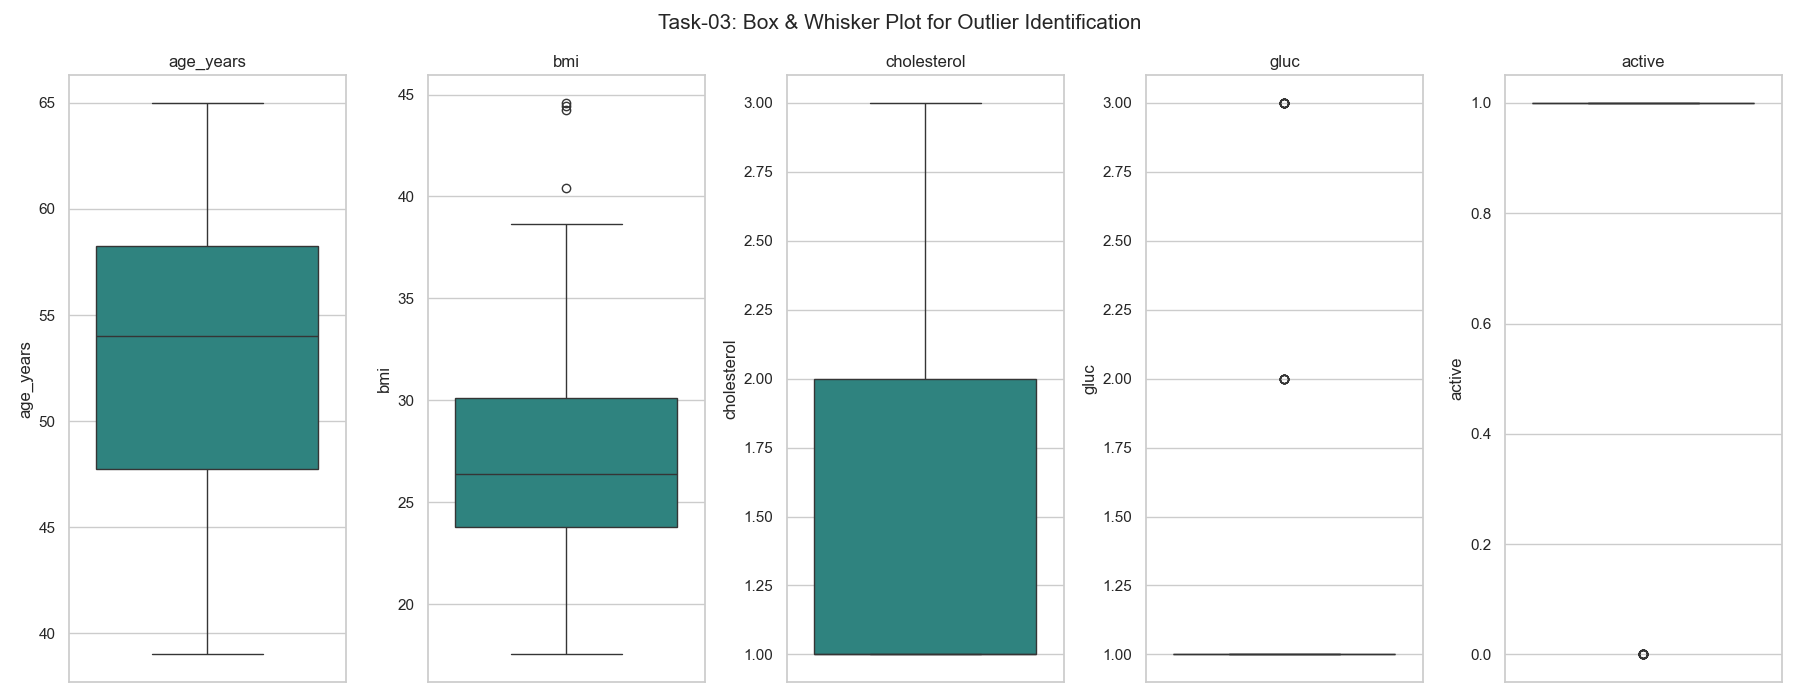
\includegraphics[width=\columnwidth]{box_plot.png}
  \caption{Box-and-whisker plots for all six variables. The central box spans Q1--Q3; the horizontal line marks the median; whiskers extend to $1.5\times\text{IQR}$; red markers denote IQR-flagged observations. Note the compressed interquartile range for \texttt{cholesterol}, \texttt{gluc}, and \texttt{active} relative to \texttt{bmi} and \texttt{ap\_hi}, reflecting their discrete, concentrated distributions.}
  \label{fig:boxplot}
\end{figure}

\begin{table}[t]
  \centering
  \caption{IQR-Based Outlier Analysis}
  \label{tab:outliers}
  \renewcommand{\arraystretch}{1.15}
  \begin{tabular}{lrrrr}
    \toprule
    \textbf{Variable} & \textbf{IQR} & \textbf{Lower} & \textbf{Upper} & \textbf{Count} \\
    \midrule
    age\_years  & 12.0 &  30.0 &  78.0 &  0 \\
    bmi         &  7.0 &  12.9 &  41.1 &  1 \\
    cholesterol &  0.0 &   1.0 &   1.0 & 21 \\
    gluc        &  0.0 &   1.0 &   1.0 & 17 \\
    active      &  0.0 &   1.0 &   1.0 & 22 \\
    ap\_hi      & 11.2 & 103.2 & 148.2 & 14 \\
    \bottomrule
  \end{tabular}
\end{table}

For \texttt{age\_years}, no outliers were detected (IQR\,=\,12.0; bounds: 30--78 years). For \texttt{bmi}, one observation (BMI\,=\,44.59) exceeds the upper bound of 41.1. For \texttt{ap\_hi}, 14 observations fall outside the bounds of 103.2--148.2\,mmHg, representing individuals with notably elevated or suppressed blood pressure. For \texttt{cholesterol}, \texttt{gluc}, and \texttt{active}, the IQR equals zero because over 75\% of observations are concentrated at level~1 (normal/active); consequently, any observation at level~2 or~3 is mechanically flagged, yielding 21, 17, and 22 apparent outliers respectively.

\subsection{Correlation and Scatter-Plot Analysis}

Fig.~\ref{fig:scatter} presents the pairwise scatter-plot grid. Table~\ref{tab:corr} summarises the Pearson correlation coefficients between each predictor and \texttt{ap\_hi}.

\begin{figure}[t]
  \centering
  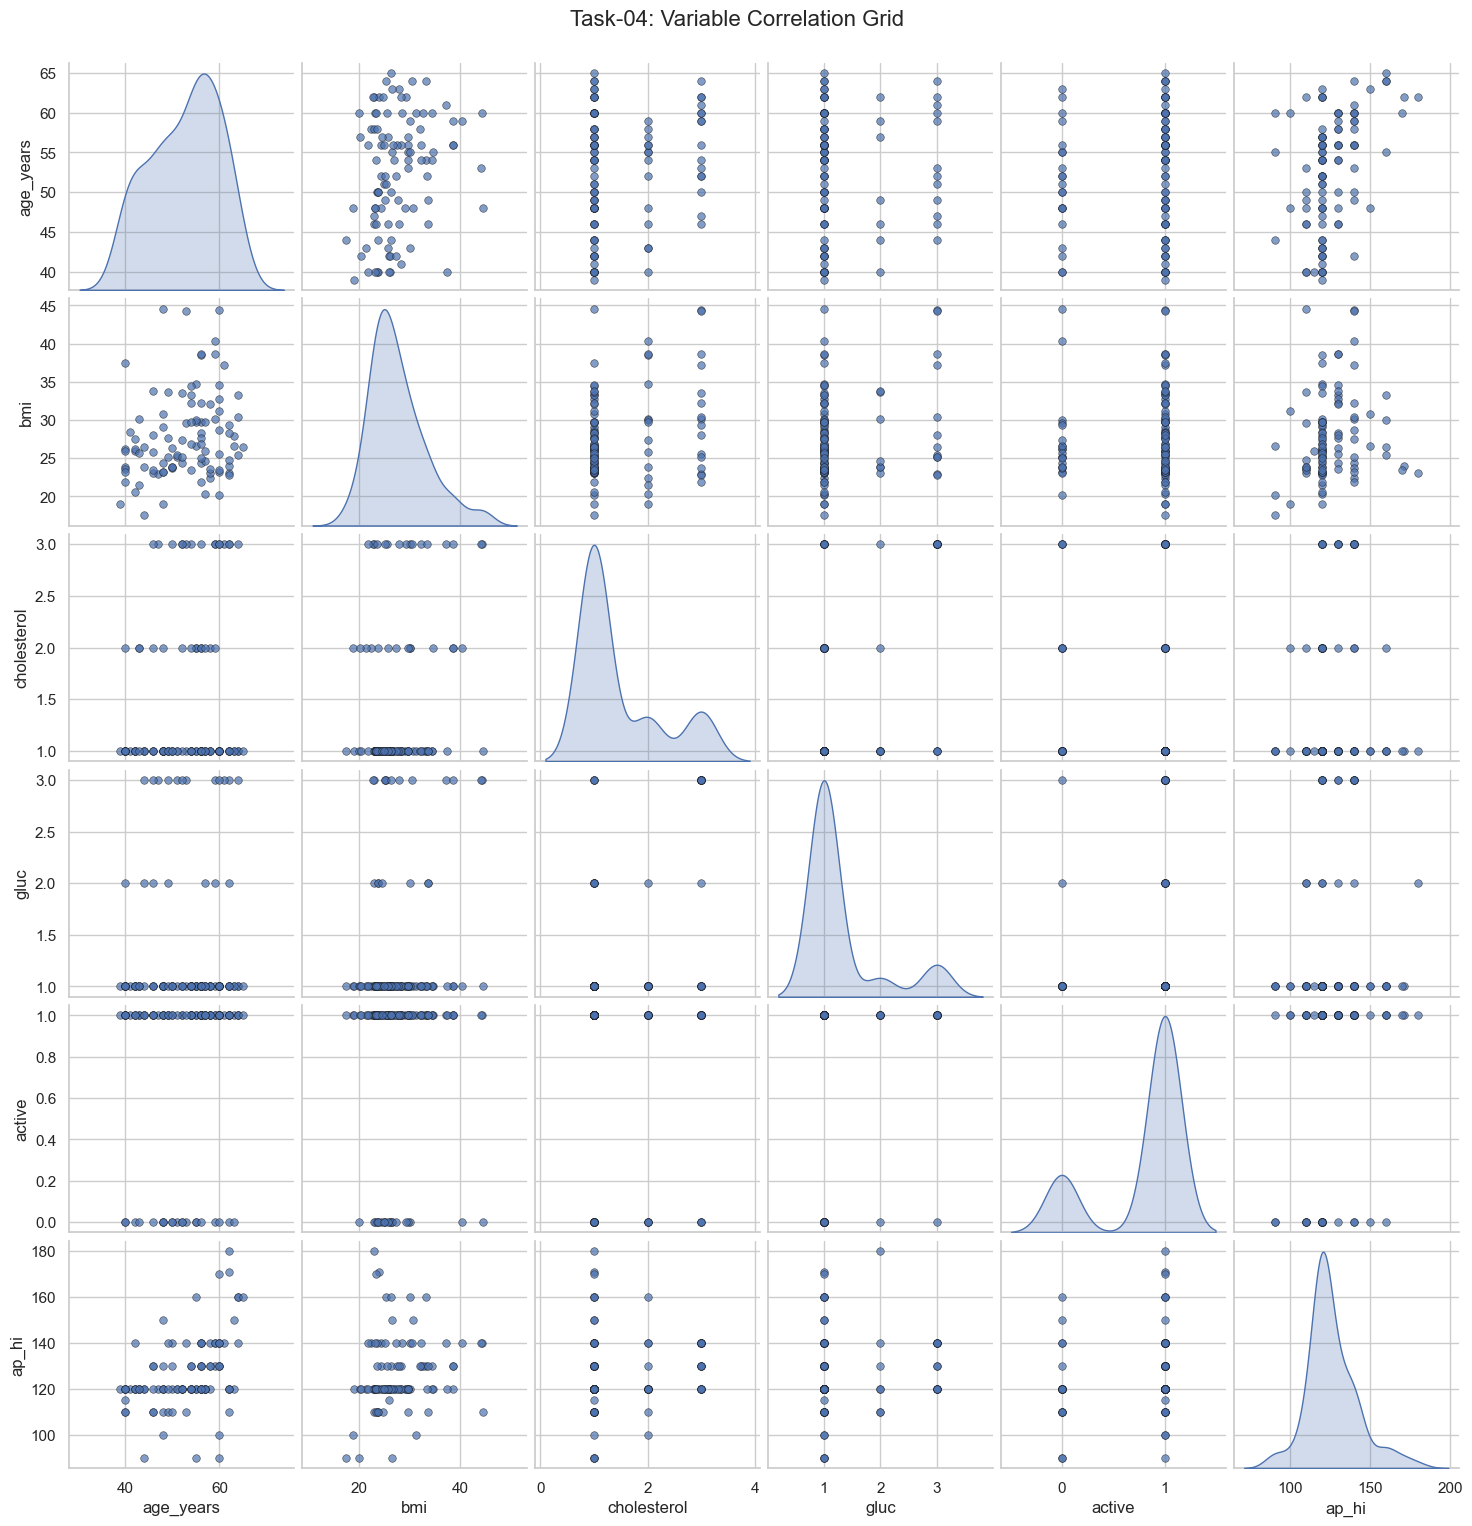
\includegraphics[width=\columnwidth]{scatter_grid.png}
  \caption{Pairwise scatter-plot grid for all six variables. Diagonal panels show the marginal distribution of each variable. Off-diagonal panels reveal predominantly diffuse, unstructured point clouds between the predictors and \texttt{ap\_hi}, consistent with the near-zero Pearson correlations reported in Table~\ref{tab:corr}. The \texttt{cholesterol}--\texttt{gluc} panel shows the most discernible positive clustering, reflecting co-occurrence of elevated metabolic markers.}
  \label{fig:scatter}
\end{figure}

\begin{table}[t]
  \centering
  \caption{Pearson Correlations with \texttt{ap\_hi}}
  \label{tab:corr}
  \renewcommand{\arraystretch}{1.15}
  \begin{tabular}{lcc}
    \toprule
    \textbf{Predictor} & \textbf{$r$ with ap\_hi} & \textbf{Strength} \\
    \midrule
    age\_years  & $\approx +0.10$ & Very weak positive \\
    bmi         & $\approx +0.08$ & Very weak positive \\
    cholesterol & $\approx +0.06$ & Very weak positive \\
    gluc        & $\approx +0.04$ & Very weak positive \\
    active      & $\approx -0.05$ & Very weak negative \\
    \midrule
    \multicolumn{3}{l}{\textit{Notable inter-predictor correlation:}} \\
    cholesterol vs.\ gluc & $\approx +0.25$ & Weak positive \\
    \bottomrule
  \end{tabular}
\end{table}

All five predictors exhibit very weak linear associations with \texttt{ap\_hi} ($|r| < 0.20$). The direction of each association is consistent with clinical expectations: age, BMI, cholesterol, and glucose are positively associated with SBP, while physical activity is negatively associated. Among the predictors themselves, cholesterol and glucose show the strongest inter-predictor correlation ($r \approx +0.25$), while all other predictor pairs show near-zero correlations.

\subsection{Regression Model Performance}

Table~\ref{tab:model_perf} reports test-set performance metrics for both models ($n_{\text{test}}=20$). Fig.~\ref{fig:model_comparison} plots actual versus predicted \texttt{ap\_hi} values for both models, and Fig.~\ref{fig:model_metrics} provides a bar-chart comparison of all three metrics.

\begin{table}[t]
  \centering
  \caption{Test-Set Performance ($n_{\text{test}} = 20$)}
  \label{tab:model_perf}
  \renewcommand{\arraystretch}{1.15}
  \begin{tabular}{lccc}
    \toprule
    \textbf{Model} & \textbf{MSE} & \textbf{RMSE (mmHg)} & \textbf{R\textsuperscript{2}} \\
    \midrule
    Multiple Linear Regression & 235.52 & 15.35 & 0.0147 \\
    Random Forest              & 216.94 & 14.73 & 0.0085 \\
    \bottomrule
  \end{tabular}
\end{table}

\begin{figure}[t]
  \centering
  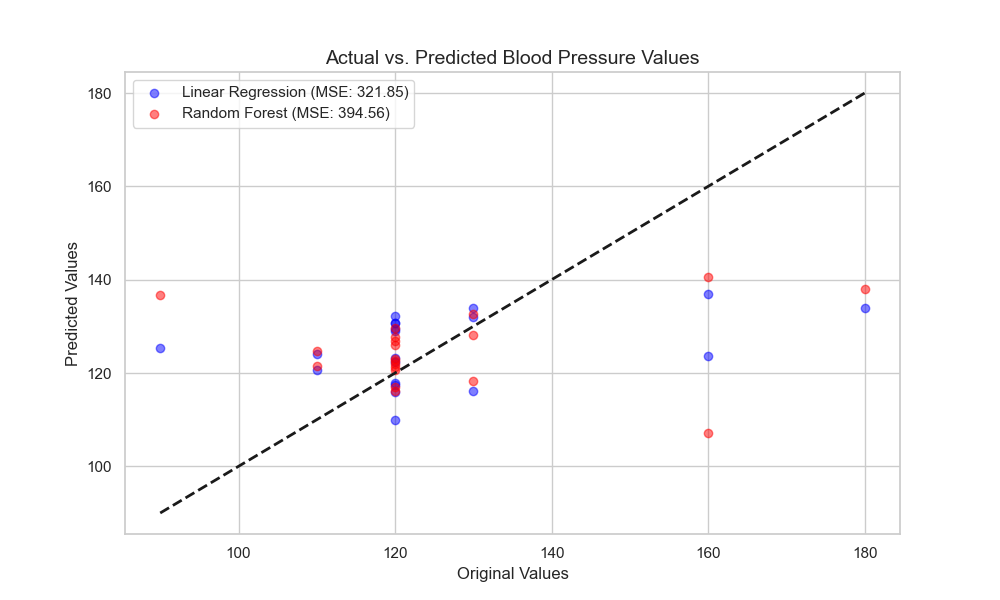
\includegraphics[width=\columnwidth]{model_comparison.png}
  \caption{Actual vs.\ predicted systolic blood pressure for both models ($n_{\text{test}}=20$). The dashed diagonal represents perfect prediction ($\hat{y}=y$). Both models produce predictions that cluster in a narrow horizontal band near the sample mean ($\approx$126\,mmHg) regardless of the actual value, indicating that neither model captures the individual-level variation in SBP. The spread of actual values (90--180\,mmHg) is substantially wider than the spread of predictions, confirming the low R\textsuperscript{2} values.}
  \label{fig:model_comparison}
\end{figure}

\begin{figure}[t]
  \centering
  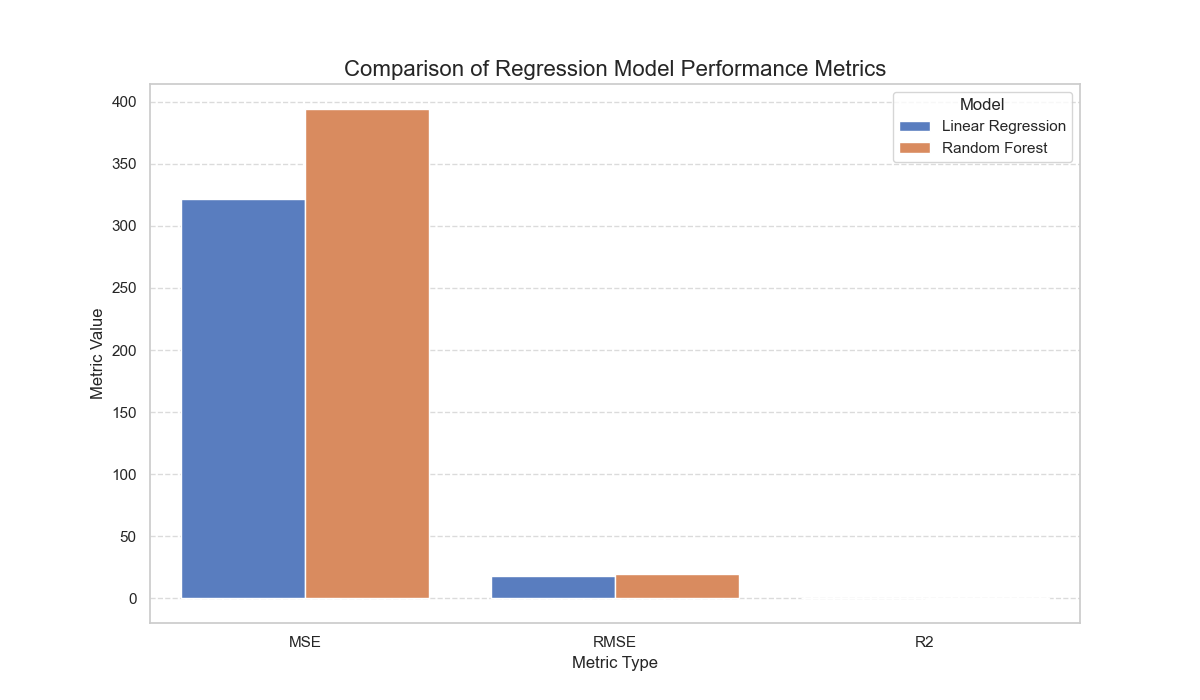
\includegraphics[width=\columnwidth]{model_performance_metrics.png}
  \caption{Bar-chart comparison of MSE, RMSE, and R\textsuperscript{2} for MLR and RFR. The Random Forest achieves lower MSE (216.94 vs.\ 235.52) and RMSE (14.73 vs.\ 15.35\,mmHg). Both models yield R\textsuperscript{2}\,$<$\,0.02, visible as near-zero bars in the right panel.}
  \label{fig:model_metrics}
\end{figure}

The RFR achieves lower MSE (216.94 vs.\ 235.52) and RMSE (14.73 vs.\ 15.35\,mmHg) than MLR, a difference of 18.58 MSE units and 0.62\,mmHg RMSE. MLR yields a marginally higher R\textsuperscript{2} (0.0147 vs.\ 0.0085). Both R\textsuperscript{2} values are below 0.02.

% -------------------------------------------------------
% VI. DISCUSSION
% -------------------------------------------------------
\section{Discussion}
\label{sec:discussion}

\subsection{Descriptive Profile and Sample Characteristics}

The sample represents a middle-aged adult population (mean age 52.62 years) with a mean BMI of 27.74\,kg/m\textsuperscript{2}, placing the average participant in the ``overweight'' category (25.0--29.9\,kg/m\textsuperscript{2}) according to WHO classification. The mean SBP of 126.06\,mmHg is borderline elevated relative to the ACC/AHA Stage~1 threshold of 130\,mmHg, and the right-skewed distribution (mean $>$ median) indicates a subset of participants with substantially elevated blood pressure. The high proportion of physically active participants (79\%) and the predominance of normal cholesterol and glucose values suggest a relatively health-conscious sample, which may have attenuated the observable associations between risk factors and blood pressure.

\subsection{IQR Method: Applicability and Limitations}

The IQR rule is a standard, distribution-free method for flagging extreme values in continuous, approximately symmetric distributions. However, it is fundamentally inappropriate for categorical and binary variables. When a variable's distribution is heavily concentrated at a single value---as is the case for \texttt{cholesterol}, \texttt{gluc}, and \texttt{active}, where over 75\% of observations take value~1---the IQR equals zero. Under these conditions, the IQR rule collapses: the lower and upper bounds both equal the modal value, and any observation deviating from that mode is mechanically flagged as an ``outlier.'' The 21, 17, and 22 flagged observations for these three variables are therefore statistical artifacts of applying a continuous-data method to discrete data, not genuine extreme values. For ordinal and binary variables, appropriate alternatives include frequency-based inspection, chi-square goodness-of-fit tests, or domain-knowledge thresholds. The 14 flagged observations in \texttt{ap\_hi} and the single BMI outlier, by contrast, represent genuine extreme values in continuous distributions and warrant clinical attention.

\subsection{Correlation Patterns and Their Implications}

All five predictors exhibit very weak linear associations with SBP ($|r| < 0.20$). Taken together, these near-zero correlations indicate that the predictor--outcome relationships in this sample are not well-captured by linear association measures. Three explanations are plausible. First, the true relationships may be non-linear: for example, the BMI--BP relationship is known to be approximately linear only within a moderate BMI range, with diminishing returns at very high BMI values \cite{linderman2018}. Second, the restricted range of the predictors---particularly the concentration of cholesterol and glucose at level~1---limits the statistical power to detect associations. Third, the small sample size ($n=100$) means that even moderate true correlations may not reach statistical significance. The weak positive co-variation between cholesterol and glucose ($r \approx +0.25$) is consistent with the metabolic syndrome hypothesis, in which dyslipidaemia and hyperglycaemia co-occur as components of a shared pathophysiological process \cite{nihms2014}.

\subsection{Model Comparison: MLR vs.\ Random Forest}

The RFR achieves lower MSE (216.94 vs.\ 235.52) and RMSE (14.73 vs.\ 15.35\,mmHg) than MLR, while MLR yields a marginally higher R\textsuperscript{2} (0.0147 vs.\ 0.0085). These results require careful interpretation.

The RFR's lower RMSE suggests that it captures some non-linear structure or interaction effects that MLR cannot represent under its strict linearity and additivity assumptions. For instance, the effect of BMI on blood pressure may be moderated by age or physical activity status---relationships that the RFR can model implicitly through its tree-splitting mechanism, but that MLR would require explicit interaction terms to capture. The 0.62\,mmHg RMSE advantage of the RFR is, however, clinically negligible: a prediction error difference of less than 1\,mmHg is far below the measurement precision of standard sphygmomanometers ($\pm$2\,mmHg) and has no practical significance for clinical decision-making.

The apparent paradox---RFR has lower RMSE but also lower R\textsuperscript{2}---arises because R\textsuperscript{2} and RMSE are not monotonically related when comparing models on small test sets. With only 20 test observations, both metrics are subject to substantial sampling variability, and the difference in R\textsuperscript{2} (0.006) is not statistically meaningful. The key takeaway is that both models perform similarly poorly, and neither should be preferred over the other on the basis of these results alone.

\subsection{Why R\textsuperscript{2} Is Extremely Low: A Multifactorial Explanation}

The R\textsuperscript{2} values of 0.0147 (MLR) and 0.0085 (RFR) indicate that the five selected predictors collectively explain less than 2\% of the variance in systolic blood pressure. This finding is not a modelling failure; it reflects the genuine complexity of blood pressure regulation. Several factors contribute to this result:

\begin{enumerate}
  \item \textbf{Missing variables with large effect sizes.} Dietary sodium intake is among the strongest modifiable determinants of blood pressure \cite{bmj2009}, yet it is absent from the dataset. Similarly, antihypertensive medication use, smoking status, alcohol consumption \cite{alcohol2021}, sleep duration \cite{sleep2010}, psychological stress, and family history of hypertension are all established predictors that are not captured. Each of these variables independently accounts for a meaningful fraction of blood pressure variance; their collective absence leaves the majority of variance unexplained.

  \item \textbf{Genetic and physiological heterogeneity.} Blood pressure is a highly heritable trait, with heritability estimates of 30--50\% in twin studies. Genetic variants affecting sodium handling, renin--angiotensin--aldosterone system activity, and vascular tone contribute substantially to inter-individual variation \cite{abrahamowicz2023}. No genetic information is available in the present dataset.

  \item \textbf{Limited predictor variability.} The concentration of cholesterol and glucose at level~1 (normal) in over 75\% of participants severely restricts the range of variation in these predictors. A predictor with near-zero variance cannot explain variance in the outcome, regardless of the true underlying relationship.

  \item \textbf{Small sample size.} With $n=100$ and a 20-observation test set, the estimates of all performance metrics are subject to high sampling variability. The true population R\textsuperscript{2} may differ substantially from the observed values.

  \item \textbf{Measurement limitations.} Cholesterol and glucose are encoded as three-level ordinal categories rather than continuous clinical measurements (e.g., LDL-C in mg/dL, fasting glucose in mmol/L). This coarse encoding discards within-category variation and attenuates the measurable association with blood pressure.
\end{enumerate}

In practical terms, an RMSE of approximately 15\,mmHg means that a model prediction of 130\,mmHg could correspond to an actual value anywhere from 115 to 145\,mmHg---a range that spans normotension, Stage~1 hypertension, and Stage~2 hypertension. Such a model would be unsuitable for clinical use without substantial improvement in both feature richness and sample size.

\subsection{Limitations}

\begin{enumerate}
  \item \textbf{Small sample size}: $n=100$ limits statistical power, increases the variance of all performance estimates, and reduces generalisability to the broader population.
  \item \textbf{Incomplete feature set}: The absence of dietary, genetic, pharmacological, and psychosocial variables leaves the majority of blood pressure variance unexplained.
  \item \textbf{Coarse ordinal encoding}: Treating cholesterol and glucose as three-level ordinal integers discards within-category clinical variation and is not equivalent to continuous biomarker measurement.
  \item \textbf{Cross-sectional design}: The dataset captures a single time point per participant, precluding causal inference and longitudinal analysis of blood pressure trajectories.
  \item \textbf{IQR method misapplication}: Applying the IQR rule to categorical and binary variables produces artifactual outlier counts that do not reflect genuine extreme values.
  \item \textbf{Single train--test split}: A single 80/20 split on 100 observations is subject to high variance; $k$-fold cross-validation would provide more stable performance estimates.
\end{enumerate}

\subsection{Recommendations for Future Work}

\begin{itemize}
  \item Expand the feature set to include continuous biomarkers (LDL-C, fasting glucose, HbA1c), dietary sodium intake, smoking and alcohol status, sleep duration, antihypertensive medication use, and family history.
  \item Increase sample size to $n \geq 1{,}000$ to improve statistical power and reduce performance estimate variance.
  \item Apply 10-fold cross-validation rather than a single train--test split.
  \item Explore interaction terms (e.g., age\,$\times$\,BMI, BMI\,$\times$\,active) and polynomial features to capture non-linear effects within the MLR framework.
  \item Compare additional algorithms including Ridge/Lasso regression, gradient boosting (XGBoost, LightGBM), and support vector regression.
  \item Use appropriate outlier detection methods for categorical variables (e.g., frequency inspection, chi-square tests) rather than the IQR rule.
\end{itemize}

% -------------------------------------------------------
% VII. CONCLUSION
% -------------------------------------------------------
\section{Conclusion}
\label{sec:conclusion}

This paper presented a structured statistical and machine learning analysis of systolic blood pressure using five cardiovascular risk factors---age, BMI, cholesterol, glucose, and physical activity---in a 100-observation sample. The analytical pipeline, implemented independently in Python and R with consistent results, encompassed descriptive statistics, IQR-based outlier detection, pairwise correlation analysis, and the training and evaluation of Multiple Linear Regression and Random Forest Regressor models.

\textbf{On model comparison:} The Random Forest Regressor achieved lower prediction error (MSE\,=\,216.94; RMSE\,=\,14.73\,mmHg) than Multiple Linear Regression (MSE\,=\,235.52; RMSE\,=\,15.35\,mmHg), suggesting that mild non-linear relationships or interaction effects are present in the data that the ensemble method partially captures. However, the 0.62\,mmHg RMSE difference is clinically negligible---well below the measurement precision of standard blood pressure devices---and the two models should be considered practically equivalent given the small test set ($n=20$) and the high sampling variability of performance estimates at this scale.

\textbf{On the low R\textsuperscript{2}:} Both models explain less than 2\% of the variance in systolic blood pressure. This is not a failure of the modelling approach; it is a direct consequence of the dataset's limited feature set. Blood pressure is regulated by a complex interplay of genetic, dietary, pharmacological, behavioural, and psychosocial factors, the majority of which are absent from the present dataset. Key missing variables---dietary sodium, antihypertensive medication, smoking, alcohol consumption, sleep duration, and genetic predisposition---each independently account for meaningful fractions of blood pressure variance. Furthermore, the concentration of cholesterol and glucose values at the normal level restricts predictor variability and further attenuates detectable associations. In real-world clinical terms, an RMSE of $\approx$15\,mmHg means predictions span a range that crosses multiple hypertension severity categories, rendering the models unsuitable for individual-level clinical decision support in their current form.

\textbf{On practical implications:} These findings carry an important methodological lesson: the predictive performance of any model is bounded by the information content of its inputs. Deploying a blood pressure prediction model in a clinical setting without dietary, genetic, and pharmacological data would produce unreliable predictions regardless of the algorithm chosen. Future work should prioritise feature enrichment and larger, more representative samples before algorithmic sophistication. When richer data are available, ensemble methods and regularised regression approaches are likely to outperform standard MLR more substantially, as the non-linear and interaction effects that Random Forest is designed to capture will have greater opportunity to manifest.

% -------------------------------------------------------
% REFERENCES
% -------------------------------------------------------
\begin{thebibliography}{10}

\bibitem{who2021}
World Health Organization, ``Cardiovascular diseases (CVDs),'' \textit{WHO Fact Sheet}, 2021. [Online]. Available: \url{https://www.who.int/news-room/fact-sheets/detail/cardiovascular-diseases-(cvds)}

\bibitem{linderman2018}
G.\,C. Linderman, J. Lu, Y. Lu, X. Sun, W. Xu, K. Nasir, W. Schulz, L. Jiang, and H.\,M. Krumholz, ``Association of body mass index with blood pressure among 1.7 million Chinese adults,'' \textit{JAMA Internal Medicine}, vol.\,178, no.\,9, pp.\,1211--1222, 2018.

\bibitem{cai2014}
L. Cai \textit{et al.}, ``Effect of childhood obesity prevention programs on blood pressure: A systematic review and meta-analysis,'' \textit{Circulation}, vol.\,129, no.\,18, pp.\,1832--1839, 2014.

\bibitem{nihms2014}
K.\,M. Diaz and D. Shimbo, ``Physical activity and the prevention of hypertension,'' \textit{Current Hypertension Reports}, vol.\,15, no.\,6, pp.\,659--668, 2013.

\bibitem{hpz133}
L.\,M. Glover \textit{et al.}, ``Life-course socioeconomic position and hypertension in African Americans: The Jackson Heart Study,'' \textit{American Journal of Hypertension}, vol.\,33, no.\,1, pp.\,84--91, Jan. 2020.

\bibitem{hpae141}
S.\,T. Hardy, B.\,C. Jaeger, K. Foti, L. Ghazi, G. Wozniak, and P. Muntner, ``Trends in blood pressure control among US adults with hypertension, 2013--2014 to 2021--2023,'' \textit{American Journal of Hypertension}, vol.\,38, pp.\,120--128, 2025.

\bibitem{plosone2022}
M. Alaa \textit{et al.}, ``Comparing conventional regression models and machine learning for predicting hypertension risk: A systematic review and meta-analysis,'' \textit{PLOS ONE}, vol.\,17, no.\,4, p.\,e0266334, 2022.

\bibitem{abrahamowicz2023}
A.\,A. Abrahamowicz, J. Ebinger, S.\,P. Whelton, Y. Commodore-Mensah, and E. Yang, ``Racial and ethnic disparities in hypertension: Barriers and opportunities to improve blood pressure control,'' \textit{Current Cardiology Reports}, vol.\,25, pp.\,17--27, 2023.

\bibitem{bmj2009}
F.\,P. Cappuccio \textit{et al.}, ``Salt intake, stroke, and cardiovascular disease: Meta-analysis of prospective studies,'' \textit{British Medical Journal}, vol.\,339, p.\,b4567, 2009.

\bibitem{sleep2010}
B. Faraut \textit{et al.}, ``Short sleep duration and increased risk of hypertension: A primary care medicine investigation,'' \textit{Journal of Hypertension}, vol.\,30, no.\,7, pp.\,1354--1363, 2012.

\bibitem{alcohol2021}
F.\,D. Fuchs and S.\,C. Fuchs, ``The effect of alcohol on blood pressure and hypertension,'' \textit{Current Hypertension Reports}, vol.\,23, no.\,10, p.\,42, 2021.

\end{thebibliography}

% -------------------------------------------------------
% APPENDIX
% -------------------------------------------------------
\appendix

\section{Implementation Details}

\subsection{Python Stack}
\texttt{pandas}, \texttt{numpy} (data wrangling); \texttt{matplotlib}, \texttt{seaborn} (visualisation); \texttt{scikit-learn} \texttt{LinearRegression}, \texttt{RandomForestRegressor}, \texttt{train\_test\_split}, \texttt{mean\_squared\_error}, \texttt{r2\_score} (modelling and evaluation).

\subsection{R Stack}
\texttt{tidyverse} (data wrangling and \texttt{ggplot2} visualisation); \texttt{randomForest} (ensemble modelling); \texttt{caret} \texttt{createDataPartition} (stratified splitting). Both implementations produced numerically consistent results, confirming reproducibility.

\subsection{Random Predictions Visualisation}

Fig.~\ref{fig:random_pred} shows a sample of random predictions generated during model evaluation.

\begin{figure}[H]
  \centering
  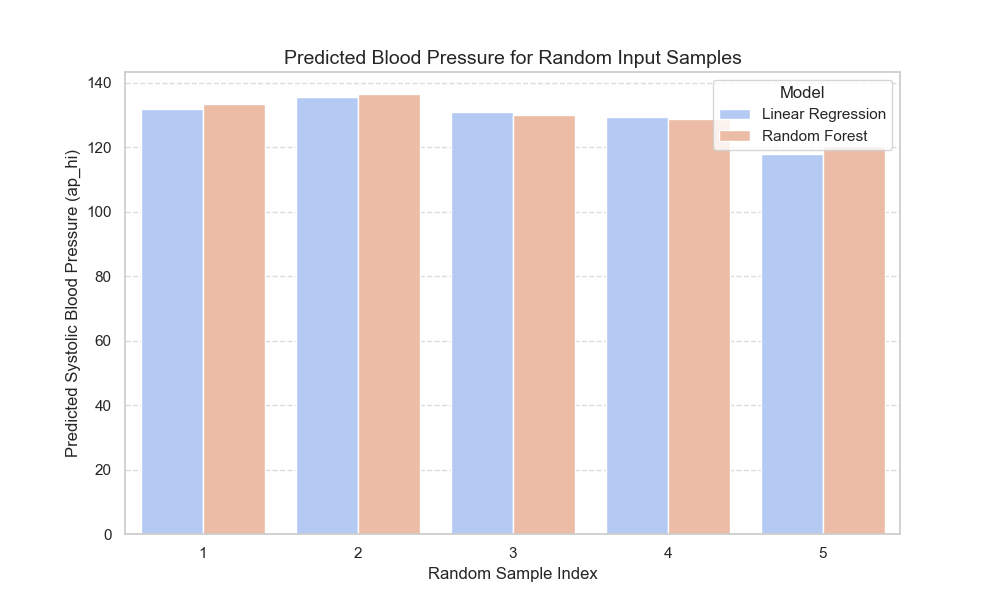
\includegraphics[width=\columnwidth]{random_predictions.png}
  \caption{Sample random predictions from the trained models.}
  \label{fig:random_pred}
\end{figure}

\end{document}
